\documentclass{article}
\usepackage[T1]{fontenc}
\usepackage{fancyhdr}
\usepackage{extramarks}
\usepackage{amsmath}
\usepackage{amsthm}
\usepackage{amsfonts}
\usepackage{dsfont}
\usepackage{tikz}
\usepackage[plain]{algorithm}
\usepackage{algpseudocode}
\usepackage{graphicx}
\usepackage{listings}
\usepackage{multicol,multirow,array,listings,tabularx,lastpage,textcomp,booktabs}
\usepackage{amssymb}
\usepackage{enumerate}
\usepackage{xcolor}
\usepackage{hyperref}

\usetikzlibrary{automata,positioning,arrows}

\graphicspath{ {./img} } 

\definecolor{light-gray}{gray}{0.95}

\lstset{numbers=right, 
        numberstyle=\tiny, 
        breaklines=true,
        backgroundcolor=\color{light-gray},
        numbersep=5pt,
        xleftmargin=.25in,
        xrightmargin=.25in,
        tabsize=4} 

\lstset{language=C++} 

%
% Basic Document Settings
%

\topmargin=-0.60in
\evensidemargin=0in
\oddsidemargin=0in
\textwidth=6.5in
\textheight=9.0in
\headsep=0.25in

\linespread{1.1}

\pagestyle{fancy}
\lhead{\hmwkAuthorName}
\chead{\hmwkTitle}
\rhead{\hmwkClass}
\lfoot{\lastxmark}
\cfoot{\thepage}

\renewcommand\headrulewidth{0.4pt}
\renewcommand\footrulewidth{0.4pt}

\setlength\parindent{0pt}
\setlength{\parskip}{5pt}

\definecolor{crimson}{HTML}{C51236}

\hypersetup{
  colorlinks=true,
  linkcolor=blue,
  filecolor=magenta,      
  urlcolor=crimson,
  pdftitle={CSE 105 Project Task 2},
  pdfpagemode=FullScreen,
}

%
% Homework Details
%   - Title
%   - Due date
%   - Class
%   - Section/Time
%   - Instructor
%   - Author
%

\newcommand{\hmwkTitle}{Project Task 2}
\newcommand{\hmwkDueDate}{Feb 22, 2024}
\newcommand{\hmwkClass}{CSE 105}
\newcommand{\hmwkClassInstructor}{Professor Minnes Kemp}
\newcommand{\hmwkAuthorName}{\textbf{Ray Tsai}}
\newcommand{\hmwkPID}{A16848188}

%
% Title Page
%

\title{
    \vspace{2in}
    \textmd{\textbf{\hmwkClass:\ \hmwkTitle}}\\
    \normalsize\vspace{0.1in}\small{Due\ on\ \hmwkDueDate\ at 5:00pm}\\
    \vspace{0.1in}\large{\textit{\hmwkClassInstructor}} \\
    \vspace{3in}
}

\author{
  \hmwkAuthorName \\
  \vspace{0.1in}\small\hmwkPID
}
\date{}

%
% Various Helper Commands
%

% Useful for algorithms
\newcommand{\alg}[1]{\textsc{\bfseries \footnotesize #1}}

% For derivatives
\newcommand{\deriv}[1]{\frac{\mathrm{d}}{\mathrm{d}x} (#1)}

% For partial derivatives
\newcommand{\pderiv}[2]{\frac{\partial}{\partial #1} (#2)}

% Integral dx
\newcommand{\dx}{\mathrm{d}x}

% Probability commands: Expectation, Variance, Covariance, Bias
\newcommand{\Var}{\mathrm{Var}}
\newcommand{\Cov}{\mathrm{Cov}}
\newcommand{\Bias}{\mathrm{Bias}}
\newcommand*{\Z}{\mathbb{Z}}
\newcommand*{\Q}{\mathbb{Q}}
\newcommand*{\R}{\mathbb{R}}
\newcommand*{\C}{\mathbb{C}}
\newcommand*{\N}{\mathbb{N}}
\newcommand*{\prob}{\mathds{P}}
\newcommand*{\E}{\mathds{E}}

\begin{document}

\maketitle

\pagebreak

\section*{Context}

In the context of UCSD's course \textit{Theory of Computability} (CSE 105), Task 2 challenges students to illustrate their understanding of deterministic finite automata (DFA) and Turing machines through practical application (see \href{https://theory-cs.github.io/output/assignments/projectCSE105W24.html#task-2-illustrating-a-theorem}{here}). Students are required to construct a DFA to recognize a specific pattern and then using that DFA as a basis to design a Turing machine that proves that the language encoding this pattern is decidable. This demonstrates decidability by establishing a Turing machine that can methodically evaluate the submission against the project's criteria.

For a submission to be considered valid, it must follow:

\begin{enumerate}[Step 1 -]
  \item Give the clear \textbf{context} and justification for the chosen application.
  \item Specify the specified \textbf{alphabet} and precise description of the \textbf{language} relevant to the application.
  \item Give \textbf{Examples} of strings within and outside the set, with explanations.
  \item Design a \textbf{DFA} that recognizes this language, with a state diagram and justification of its functionality.
  \item Construct a \textbf{Turing machine} based on the DFA, with additional states as required.
  \item Give an illustration of the Turing machine's \textbf{computation} on a selected string from the DFA.
\end{enumerate}

In this task, we will design a DFA that assess whether a submission adheres to the task's specified guidelines. Subsequently, this DFA will serve as the foundation for constructing a Turing machine, which will establish that the language encoding the chosen pattern is indeed decidable. If the submission correctly fulfills all criteria, the Turing machine will accept it; if not, it will be rejected. The choice of this application is due to its direct relation to a project in the \textit{Theory of Computability} (CSE 105) course that I am currently enrolled in and \textbf{care about a lot}.

\section*{Alphabet and Language}

For this application, we will use the alphabet $\Sigma = \{(CON), (AL), (EX), (DFA), (TM), (COMP)\}$, with each symbol representing an abbreviation for the initial letters of the key components in each task step: $(CON)$ for context, $(AL)$ for alphabet and language, $(EX)$ for example, $(DFA)$ for DFA, $(TM)$ for Turing machine, and $(COMP)$ for computation.

The language encoding our chosen pattern is described by the regular expression
\[
  R = (CON)^+(AL)(EX)^2(DFA)(TM)(COMP).
\]
The expression $R$ specifies a sequence of setps where each of the six steps must appear at least once and in the correct order. The use of the plus sign (+) after $(CON)$ indicates that these steps can be repeated one or more times, reflecting their potential multiple occurrences (paragraphs) in a project submission. 

\section*{$\text{Example}^2$}

An example within $L(R)$ is $w = (CON)(AL)(EX)(EX)(DFA)(TM)(COMP)$, representing the minimal sequence for a valid submission, containing all essential components in the correct order. Conversely, $s = (CON)(AL)(EX)(EX)$ is not in $L(R)$. The choice of $s$ is due to its reflection of our current progress. Since we have not completed the task, $s$ illustrates an invalid submission, and thus $s \notin L(R)$.
 
\section*{DFA}

We now design a DFA $M$ that recognizes $L(R)$.
\begin{center}
  State diagram of $M$

  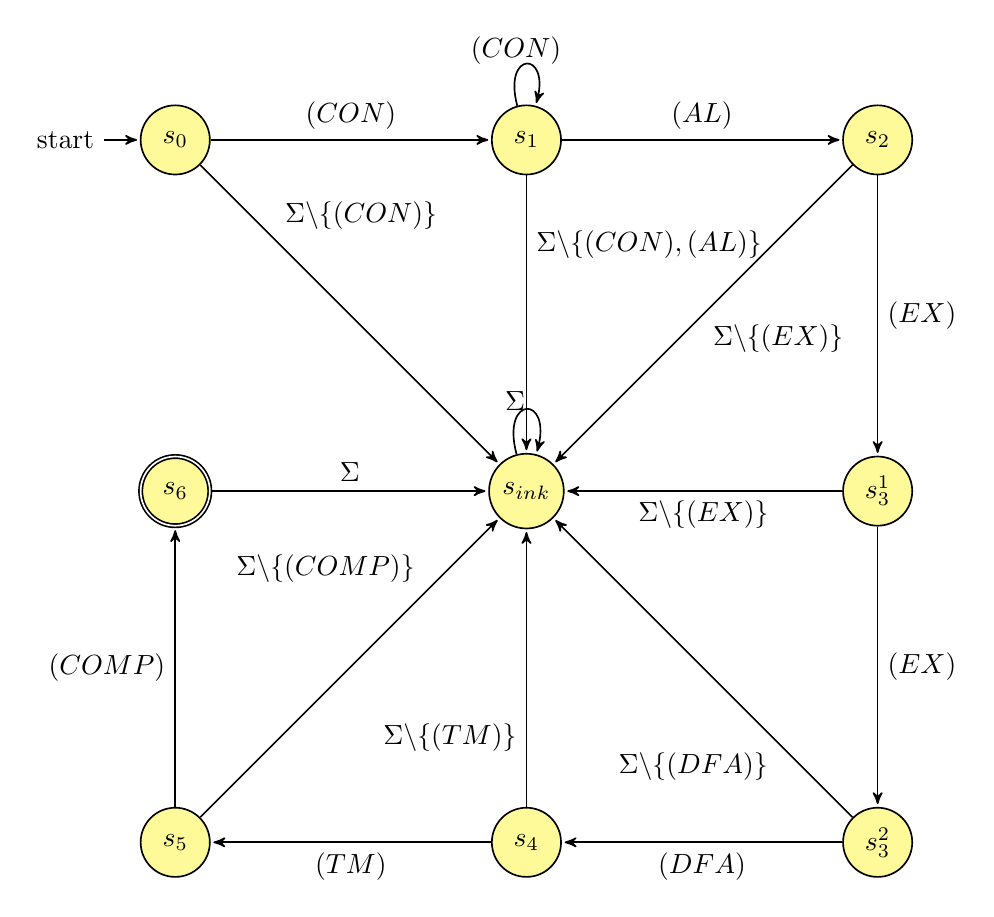
\begin{tikzpicture}[->,>=stealth',shorten >=1pt, auto, node distance=2cm, semithick]
    \tikzstyle{every state}=[text=black, fill=yellow!40]
    
    \node[initial,state] (s_0)          {$s_0$}; \node[state] (s_1) [right of=s_0, xshift=70pt] {$s_1$}; \node[state] (s_2) [right of=s_1, xshift=70pt] {$s_2$}; \node[state] (s_31) [below of=s_2, yshift=-70pt] {$s_3^1$}; \node[state] (s_32) [below of=s_31, yshift=-70pt] {$s_3^2$}; \node[state] (s_4) [left of=s_32, xshift=-70pt] {$s_4$}; \node[state] (s_5) [left of=s_4, xshift=-70pt] {$s_5$}; \node[state, accepting] (s_6) [above of=s_5, yshift=70pt] {$s_6$}; \node[state] (sink) [right of=s_6, xshift=70pt] {$s_{ink}$};

    \path (s_0) edge  [] node {$(CON)$} (s_1) (s_1) edge  [loop above, near start] node {$(CON)$} (s_1) (s_1) edge  [] node {$(AL)$} (s_2) (s_2) edge  [] node {$(EX)$} (s_31) (s_31) edge [] node {$(EX)$} (s_32) (s_32) edge [] node {$(DFA)$} (s_4) (s_4) edge  [] node {$(TM)$} (s_5) (s_5) edge  [] node {$(COMP)$} (s_6) (sink) edge  [loop above, near start] node {$\Sigma$} (sink)

          (s_0) edge  [near start] node {$\Sigma \backslash \{(CON)\}$} (sink) (s_1) edge  [near start] node {$\Sigma \backslash \{(CON), (AL)\}$} (sink) (s_2) edge  [] node {$\Sigma \backslash \{(EX)\}$} (sink) (s_31) edge [] node {$\Sigma \backslash \{(EX)\}$} (sink) (s_32) edge [near start] node {$\Sigma \backslash \{(DFA)\}$} (sink) (s_4) edge  [near start] node {$\Sigma \backslash \{(TM)\}$} (sink) (s_5) edge  [near end] node {$\Sigma \backslash \{(COMP)\}$} (sink) (s_6) edge  [] node {$\Sigma$} (sink) ;
    \end{tikzpicture}
\end{center}

The DFA $M$ is designed with a set of states $Q = \{s_0, s_1, s_2, s_3^1, s_3^2, s_4, s_5, s_6, s_{ink}\}$. Each state $s_i$ corresponds to a specific step in the validation sequence of the input string, with $s_0$ as the initial state. Note that $s_3^1, s_3^2$ represents the number of $(EX)$ recieved from the input string. In addition, the $s_{ink}$ state is a non-accepting state that absorbs any string deviating from the language's specified sequence. Transitions from each state to the $s_{ink}$ state occur upon reading an input not expected at that stage, ensuring that only strings following the exact order of components $(CON)^+(AL)(EX)^2(DFA)(TM)(COMP)$ are accepted.

See next page for the construciton of a Turing machine which decides $L(R)$.

\newpage

\section*{Turing Machine}

Here is the resulting $T$ following the construction in the proof of Theorem 4.1:

\begin{center}
  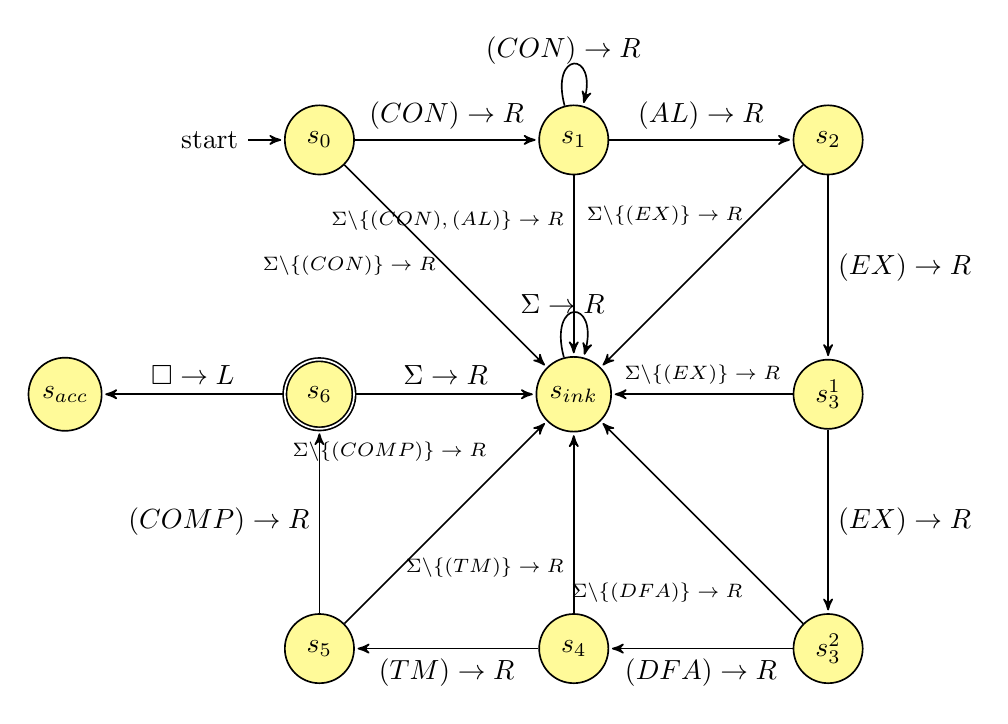
\begin{tikzpicture}[->,>=stealth',shorten >=1pt, auto, node distance=2cm, semithick]
    \tikzstyle{every state}=[text=black, fill=yellow!40]
    
    \node[initial,state] (s_0)          {$s_0$}; \node[state] (s_1) [right of=s_0, xshift=35pt] {$s_1$}; \node[state] (s_2) [right of=s_1, xshift=35pt] {$s_2$}; \node[state] (s_31) [below of=s_2, yshift=-35pt] {$s_3^1$}; \node[state] (s_32) [below of=s_31, yshift=-35pt] {$s_3^2$}; \node[state] (s_4) [left of=s_32, xshift=-35pt] {$s_4$}; \node[state] (s_5) [left of=s_4, xshift=-35pt] {$s_5$}; \node[state, accepting] (s_6) [above of=s_5, yshift=35pt] {$s_6$}; \node[state] (s_{acc}) [left of=s_6, xshift=-35pt] {$s_{acc}$}; \node[state] (sink) [right of=s_6, xshift=35pt] {$s_{ink}$};

    \path (s_0) edge  [] node {$(CON) \to R$} (s_1) (s_1) edge  [loop above, near start] node {$(CON) \to R$} (s_1) (s_1) edge  [] node {$(AL) \to R$} (s_2) (s_2) edge  [] node {$(EX) \to R$} (s_31) (s_31) edge [] node {$(EX) \to R$} (s_32) (s_32) edge [] node {$(DFA) \to R$} (s_4) (s_4) edge  [] node {$(TM) \to R$} (s_5) (s_5) edge  [] node {$(COMP) \to R$} (s_6) (s_6) edge  [above] node {$\square \to L$} (s_{acc}) (sink) edge  [loop above, near start] node {$\Sigma \to R$} (sink)

          (s_0) edge  [left] node {\scriptsize $\Sigma \backslash \{(CON)\} \to R$} (sink) (s_1) edge  [left, near start] node {\scriptsize $\Sigma \backslash \{(CON), (AL)\} \to R$} (sink) (s_2) edge  [left, near start] node {\scriptsize $\Sigma \backslash \{(EX)\} \to R$} (sink) (s_31) edge [above] node {\scriptsize $\Sigma \backslash \{(EX)\} \to R$} (sink) (s_32) edge [near start] node {\scriptsize $\Sigma \backslash \{(DFA)\} \to R$} (sink) (s_4) edge  [near start] node {\scriptsize $\Sigma \backslash \{(TM)\} \to R$} (sink) (s_5) edge  [near end] node {\scriptsize $\Sigma \backslash \{(COMP)\} \to R$} (sink) (s_6) edge  [] node { $\Sigma \to R$} (sink) ;
    \end{tikzpicture}
\end{center}

Note that, additional to $Q$, $T$ also contains $s_{acc}$ and $s_{rej}$. However, we have omitted the appearance of $s_{rej}$ and all edges associated with it from the daigram, due to the convention.

\section*{Computation}

We show the computation of string $w$ from Step 3 in $T$. Note that $w$ reflects our current progress of task 2.

\begin{center}
  \begin{tabular}{|c|c|c|c|c|c|c|c|}
    \hline
    \multicolumn{1}{|c}{$s_0\downarrow$} &  \multicolumn{7}{c|}{\phantom{A}}\\
    \hline
    $(CON)$ & $(AL)$  & $(EX)$ & $(EX)$ & ($DFA$) & ($TM$) & ($COMP$) & $\square$\\
    \hline
    \multicolumn{1}{|c}{\phantom{A}} & \multicolumn{1}{c}{$s_1\downarrow$} & \multicolumn{6}{c|}{\phantom{A}}\\
    \hline
    $(CON)$ & $(AL)$  & $(EX)$ & $(EX)$ & ($DFA$) & ($TM$) & ($COMP$) & $\square$\\
    \hline
    \multicolumn{2}{|c}{\phantom{A}} & \multicolumn{1}{c}{$s_2\downarrow$} & \multicolumn{5}{c|}{\phantom{A}}\\
    \hline
    $(CON)$ & $(AL)$  & $(EX)$ & $(EX)$ & ($DFA$) & ($TM$) & ($COMP$) & $\square$\\
    \hline
    \multicolumn{3}{|c}{\phantom{A}} & \multicolumn{1}{c}{$s_3^1\downarrow$} & \multicolumn{4}{c|}{\phantom{A}}\\
    \hline
    $(CON)$ & $(AL)$  & $(EX)$ & $(EX)$ & ($DFA$) & ($TM$) & ($COMP$) & $\square$\\
    \hline
    \multicolumn{4}{|c}{\phantom{A}} & \multicolumn{1}{c}{$s_3^2\downarrow$} & \multicolumn{3}{c|}{\phantom{A}}\\          
    \hline
    $(CON)$ & $(AL)$  & $(EX)$ & $(EX)$ & ($DFA$) & ($TM$) & ($COMP$) & $\square$\\
    \hline
    \multicolumn{5}{|c}{\phantom{A}} & \multicolumn{1}{c}{$s_4\downarrow$} & \multicolumn{2}{c|}{\phantom{A}}\\          
    \hline
    $(CON)$ & $(AL)$  & $(EX)$ & $(EX)$ & ($DFA$) & ($TM$) & ($COMP$) & $\square$\\
    \hline
    \multicolumn{6}{|c}{\phantom{A}} & \multicolumn{1}{c}{$s_5\downarrow$} & \multicolumn{1}{c|}{\phantom{A}}\\          
    \hline
    $(CON)$ & $(AL)$  & $(EX)$ & $(EX)$ & ($DFA$) & ($TM$) & ($COMP$) & $\square$\\
    \hline
    \multicolumn{7}{|c}{\phantom{A}} & \multicolumn{1}{c|}{$s_{6}\downarrow$} \\          
    \hline
    $(CON)$ & $(AL)$  & $(EX)$ & $(EX)$ & ($DFA$) & ($TM$) & ($COMP$) & $\square$\\
    \hline
    \multicolumn{6}{|c}{\phantom{A}} & \multicolumn{1}{c}{$s_{acc}\downarrow$} & \multicolumn{1}{c|}{\phantom{A}}\\          
    \hline
    $(CON)$ & $(AL)$  & $(EX)$ & $(EX)$ & ($DFA$) & ($TM$) & ($COMP$) & $\square$\\
    \hline
  \end{tabular}
\end{center}
\end{document}